\documentclass{article}
\renewcommand*\familydefault{\sfdefault}
\usepackage[utf8]{inputenc}
\usepackage[T1]{fontenc}
\setlength{\textwidth}{481pt}
\setlength{\textheight}{650pt}
\setlength{\headsep}{10pt}
\usepackage{amsfonts}
\usepackage[T1]{fontenc}
\usepackage{palatino}
\usepackage{calrsfs}
\usepackage{geometry}
\geometry{ left=3cm, top=2cm, bottom=2cm, right=2cm}
\usepackage{xcolor}
\usepackage{amsmath}
\usepackage{tikz,tkz-tab}
\usepackage{cancel}
\usepackage{pgfplots}
\usepackage{pstricks-add}
\usepackage{pst-eucl}
\usepackage{amssymb}
\usepackage{icomma}
\begin{document}
\title{Démonstration kholle 11}
\date{}
\maketitle
	\renewcommand{\thesection}{\Roman{section}}
	\setlength{\parindent}{1.5cm}
\section{Première question de cours}
\subsection{Suites récurrentes linéaires d'ordre 2 : cas complexe et discriminant $\neq 0$}
\textcolor{green}{Propriété:}
On définit un suite linéaire d'ordre 2 une suite sous la forme : \\ 
$\forall n \in \mathbb{N},u_{n+2}=au_{n+1}+bu_n$ \\ 
Si l'équation $z^2=az+b$ admet 2 racines simples $r$ et $s$ \\ 
Les suites convenant sont des combinaisons linéaires de $(r^n)_{n \in \mathbb{N}}$ et $(s^n)_{n \in \mathbb{N}}$ donc de la forme: \\ 
$\forall n \in \mathbb{N},u_n= \lambda r^n+\mu s^n$ \\ 
avec $(\lambda,\mu) \in \mathbb{C}^2$ uniquement déterminé par $u_0$ et $u_1$ \\ 
\textcolor{red}{Démonstration:} \\ 
\textcolor{green}{a)} Ces suites conviennent : \\ 
Si $u_n= \lambda r^n+\mu s^n$ pour tout $n \in \mathbb{N}$ : \\ 
$a u_{n+1}+bu_n= \lambda r^n\underbrace{(ar+b)}_{=r^2} + \mu s^n\underbrace{(as+b)}_{=s^2}$ \\ 
$r^{n+2}+s^{n+2}=u_{n+2}$ \\ 
\textcolor{green}{b)} Soit $u_n$ tel que : \\ 
$\forall n \in \mathbb{N},u_{n+2}=au_{n+1}+bu_n$ \\ 
Posons pour $n \in \mathbb{N}$: \\ 
$v_n=u_{n+1}-ru_n$ \\ 
$w_n=u_{n+1}-su_n$ \\ 
Alors :  \\ 
$v_{n+1}-sv_n=(u_{n+2}-ru_{n+1}-s(u_{n+1}-ru_n))$ \\ 
$v_{n+1}-sv_n=u_{n+2}-\underbrace{(r+s)}_{a}u_{n+1}+\underbrace{rs}_{-b}u_n$ \\ 
$v_{n+1}-sv_n= u_{n+2}-au_{n+1}-bu_n$ \\ 
$v_{n+1}-sv_n=0$ \\ 
donc : \\ 
$\forall n \in \mathbb{N},v_n=v_0s^n$ \\ 
De même avec $w_n$: \\ 
$\forall n \in \mathbb{N},w_n=w_0r^n$ \\ 
Enfin pour $n \in \mathbb{N}$: \\ 
$v_n-w_n=\underbrace{(s-r)}_{\neq 0}u_n$ \\ 
$u_n=\frac{u_n-w_n}{s-r}$ \\ 
$u_n=\underbrace{\frac{-w_0}{s-r}}_{\lambda}r^n+ \underbrace{\frac{v_0}{s-r}}_{\mu}s^n$ \\ 
\textcolor{green}{c)} $\lambda + \mu =u_0$ \\ 
$\lambda r +\mu s = u_1$ \\ 
donc $ru_0-u_1:\mu\underbrace{(r-s)}_{\neq 0}$ \\ 
$\mu=\frac{ru_0-u_1}{r-s}$ \\ 
de même avec $\lambda$ : \\ 
$su_0-u_1=\frac{su_0-u_1}{s-r}$
\subsection{Suites récurrentes linéaires d'ordre 2 : cas complexe et discriminant $= 0$}
\textcolor{green}{Propriété :} \\ 
Si l'équation caractéristique de la suite admet une racine double$r_0 \neq 0$, $u_n$ peut se mettre sous la forme : \\ 
$\forall n \in \mathbb{N}, u_n=(\lambda + \mu n){r_0}^n$ \\ 
avec $(\lambda, \mu) \in \mathbb{C}^2$ uniquement déterminé par $u_0$ et $u_1$ \\
\textcolor{red}{Démonstration :} \\ 
\textcolor{green}{a)} $\forall n \in \mathbb{N},u_n=(\lambda + \mu n){r_0}^n$ \\ 
avec $(\lambda ,\mu) \in \mathbb{C}^2$ : \\ 
Pour $n \in \mathbb{N}$ : \\ 
$au_{n+1}+bu_{n}=a \lambda {r_0}^{n+1}+a\mu (n+1){r_0}^{n+1}+b \lambda {r_0}^n+b \mu n {r_0}^n$ \\ 
$au_{n+1}+bu_{n}=\lambda {r_0}^n\underbrace{(ar_0+b)}_{r^2}+ \mu {r_0}^n(\underbrace{a}_{2r_0}(n+1)r_0+\underbrace{b}_{{r_0}^2}n$ \\ 
$au_{n+1}+bu_{n}=\lambda {r_0}^{n+2}+ \mu {r_0}^{n+2} \mu (n+2)=u_{n+2}$ \\ 
\textcolor{green}{b)} Soit $(u_n)$ tel que : \\ 
$\forall n \in \mathbb{N}, u_{n+2}=2r_0u_{n+1}-{r_0}^2u_n$ \\ 
Posons pour $n \in \mathbb{N}: x_n=\frac{u_n}{{r_0}^n}$ (licite $r_0 \neq 0$) \\ 
On a, puisque $a=2r_0$ et $-b={r_0}^2$ : \\ 
$\forall n \in \mathbb{N}, u_{n+1}=2r_0u_{n+1}-{r_0}^2u_n$ \\ 
on a donc  en divisant par ${r_0}^{n+2}$: $x_{n+2}=2x_{n+1}-x_n$ \\ 
$x_{n+2}-x_{n+1}=x_{n+1}-x_n$ \\ 
donc $x_{n+1}-x_n$ est constante donc $(x_n)$ est arithmétique : \\ 
$\exists(\lambda, \mu) \in \mathbb{C}^2, \forall n \in \mathbb{N},x_n=\lambda+ \mu n$ \\ 
$u_n=(\lambda+ \mu n){r_0}^n$ \\ 
\textcolor{green}{c)} $ \lambda = u_0$ \\ 
$(\lambda + \mu n)r_0=u_1$
donc $\mu = \frac{u_1}{r_0}-u_0$
\subsection{Cas réel à partir du cas complexe dans le cas d'un discriminant < 0}
\textcolor{green}{Propriété :} \\ 
Si l'équation caractéristique a deux racines complexes non réelle conjugées écrivons les $e^{\pm i \theta}$. \\ 
Les suites sont de la formes : \\ 
$\forall n \in \mathbb{N}, u_n=p^n(C\cos(n\theta)+D\sin(n\theta))$ \\ 
avec $(C,D) \in \mathbb{R}^2$ déterminé par $u_0$ et $u_1$ \\ 
\textcolor{red}{Démonstration :} \\
$\exists(\lambda, \mu) \in \mathbb{C}^2, \forall n \in \mathbb{N}, u_n=\lambda(pe^{i\theta})^n+ \mu (pe^{-i \theta})^n$ \\ 
conjuguons : \\ 
$\forall n \in \mathbb{N}, u_n \in \mathbb{R}, u_n=\bar{\lambda}(pe^{-i \theta})^n+ \bar{\mu}(pe^{i\theta})$ \\ 
Donc par unicité des coefficients : \\
$\lambda=\bar{\mu}$
Notons $ \mu= B e^{i \phi}(B \in \mathbb{R}_+, \phi \in \mathbb{R})$ \\ 
Pour $n \in \mathbb{N}$ : \\ 
$u_n=Be^{-i \phi}p^ne^{in\theta}+B e^{i\phi }p^ne^{-in\theta}$ \\ 
$u_n=2Bp^n\cos(n\theta- \phi)$ \\ 
$u_n=p^n(\underbrace{2B\cos(\phi)}_{C\in \mathbb{R}}cos(n\theta)+\underbrace{2Bsin(\phi)}_{D\in \mathbb{R}}sin(n\theta))$ \\ 
ensuite: $u_0=c$ \\ 
$u_1=p(Ccos(\theta)+Dsin(\theta))$ \\ 
$D=\frac{u_1-pCcos(\theta)}{p sin(\theta)}$ \\ 
licite car $p>0$ et $\theta \not\equiv 0[\pi]$ car racines $\notin \mathbb{R}$ \\ 
\subsection{Etude de la suite récurrentes $u_{n+1}= \sqrt{1+u_n}$ avec illustration graphique}
Soit la suite suivante : \\ 
$u_{n+1}=\sqrt{(1+u_n)}$ \\ 
$I=[-1,+\infty[$ \\ 
$f:I \rightarrow \mathbb{R}_+$ \\ 
$x \rightarrow \sqrt{1+x}$ \\ 
I stable donc, avec $u_0\in I$ \\ 
Posons $g : I \rightarrow \mathbb{R}$ \\ 
$x \rightarrow f(x)-x$ \\ 
$\forall x \in I, g'(x)=\frac{1}{2\sqrt{1+x}}-1$ \\ 
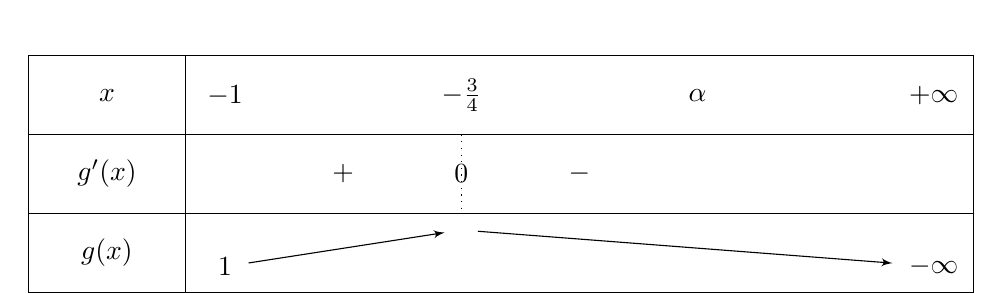
\begin{tikzpicture}
\tkzTabInit{$x$ / 1 , $g'(x)$ / 1, $g(x)$ / 1 }{$-1$, $-\frac{3}{4}$,$\alpha$, $+\infty$}
\tkzTabLine{, +, z, -,} 
 \tkzTabVar{-/ $1$,  +/ $$,  R/,-/ $-\infty$,}
\end{tikzpicture}
\\
Après étude du tableau de variation on voit : \\ 
$\exists ! \alpha \in I, g(\alpha)=0$ c'est-à-dire $f(\alpha)=\alpha$ \\ 
Calculons $\alpha$: \\ 
$\sqrt{1+ \alpha}= \alpha$ \\ 
$\alpha^2-\alpha-1=0$ \\ 
$\alpha=\frac{1+\sqrt{5}}{2}$ ou $\alpha=\frac{1-\sqrt{5}}{2}$ \\ 
Or $\alpha=\sqrt{1+\alpha} \geq 0$ donc $\alpha=\frac{1+\sqrt{5}}{2}$ \\
On voit d'après la réprésentation graphique : \\ 
Si $u_0 \in [-1;\alpha[$ \\ 
Comme f est strictement croissante ; \\ 
$\forall n \in \mathbb{N},u_n \in [-1,\alpha[$ \\ 
Si $-1 \leq u_n \leq \alpha$ \\ 
$-1\leq f(-1) \leq \underbrace{f(u_n)}_{u_{n+1}} \leq f(\alpha)=\alpha$ \\ 
Pour $n \in \mathbb{N}$: \\ 
$u_{n+1}-u_n=g(u_n)>0$ car $u_n \in [-1,\alpha[$\\
donc $u_n$ strictement croissante
Par le théorèmes de la limite monotone : \\ 
$u_n$ converge \\ 
la limite l est telle que $l=\sqrt{1+l}$ c'est-à-dire $f(l)=l$ donc $l=\alpha$
donc $u_n \rightarrow \alpha$ \\ 
Si$u_0= \alpha$ \\ 
Alors $\forall n \in \mathbb{N},u_n= \alpha$ \\ 
Si $u_0>\alpha$
Comme f est strictement croissante : \\ 
$\forall n \in \mathbb{N}, u_n > \alpha$ \\ 
En effet, si $u_n> \alpha$ \\
$u_{n+1}=f(u_n)\geq f(\alpha)=\alpha$ \\ 
Pour $n \in \mathbb{N}$ : \\ 
$u_{n+1}-u_n=g(u_n)<0$ donc $u_n$ est croissante \\ 
or $u_n> \alpha$ \\ 
Par le théorème de la limite monotone : \\ 
on obtient $u_n \rightarrow \alpha$
\subsection{Etude de la suite récurrentes $u_{n+1}= \frac{1}{1+u_n}$ avec illustration graphique}
On a : \\ 
$u_0>-1$ \\ 
$\forall n \in \mathbb{N},u_{n+1}=\frac{1}{1+u_n}$ \\ 
Avec $I=]-1; +\infty[$ et : \\
$f: I \rightarrow \mathbb{R}$ \\ 
$x \rightarrow \frac{1}{1+x}$ \\ 
Posons $h= f of$ h est strictement croissante car f est strictement décroissante \\ 
Posons $v_n=u_{2n}$ et $w_n=u_{2n+1}$ pour $n \in \mathbb{N}$ : \\ 
$\forall n \in \mathbb{N},v_{n+1}=h(v_n)$ et $\forall n \in \mathbb{N},w_{n+1}=h(w_n)$ \\ 
Pour $x \in  I$ : $h(x)=\frac{1}{1+\frac{1}{1+x}}=\frac{1+x}{2+x}$ \\ 
Posons $g(x): x \in I \rightarrow h(x)-x=\frac{1-x-x^2}{2+x}$ \\ 
or $g(x)=1-\frac{1}{2+x}-x$ \\ 
d'où : $g'(x)=\frac{1}{(2+x)^2}-1$ \\ 
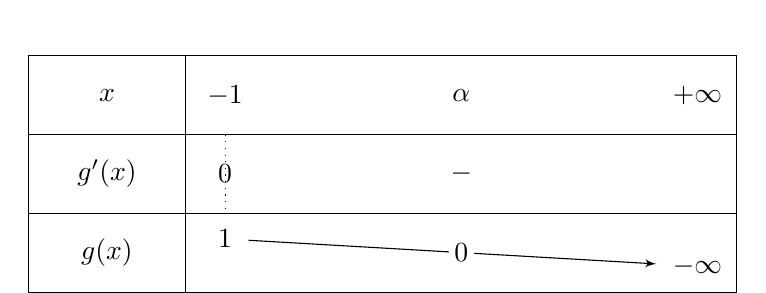
\begin{tikzpicture}
\tkzTabInit{$x$ / 1 , $g'(x)$ / 1, $g(x)$ / 1 }{$-1$, $\alpha$, $+\infty$}
\tkzTabLine{ z, , -,} 
 \tkzTabVar{+/ $1$,  R/,-/ $-\infty$,}
 \tkzTabIma{1}{3}{2}{$0$}
\end{tikzpicture}
On trouve comme solution pour g(x)=x : \\ 
$\alpha=\frac{-1+\sqrt{5}}{2}$ ou $\alpha=\frac{1-\sqrt{5}}{2}<-1$ donc $\alpha=\frac{-1+\sqrt{5}}{2}$ \\ 
Si $u_0<a$ : \\ 
$v_0=u_0< \alpha$ \\ 
Comme h strictement croissante : $\forall n \in \mathbb{N},v_n<\alpha$ \\
Comme $g>0$ sur $]-1;\alpha[$ $v_n$ est strictement croissante \\ 
Théorème de la limite monotone : \\ 
Soit $l=\lim_{n \rightarrow + \infty}(v_n)\in \mathbb{R}$ alors $h(l)=l$ $l=\alpha$ donc : \\ 
$v_n \rightarrow \alpha$ \\ 
$w_0=u_1=f(u_0)>f(\alpha)=\alpha$ \\ 
Comme h est strictement croissante $\forall n \in \mathbb{N}, w_n>a$ \\ 
Comme $g<0$ sur $]\alpha;+\infty[$ $(w_n)$ strictement décroissante \\ 
donc $w_n$ converge vers $\alpha$ \\ 
Commme $u_{2n}\rightarrow \alpha$ et $u_{2n+1} \rightarrow \alpha$ donc $u_n \rightarrow \alpha$  \\ 
Si $u_0=\alpha : \forall n\in \mathbb{N}, u_n=\alpha$ \\ 
Si $u_0>\alpha$: comme si $u_0<\alpha$ en intervertissant les roles de $u_n$ et $v_n$ : $u_n \rightarrow \alpha$
\section{Deuxième question de cours}
\subsection{Neuf définitions quantifiées de la définition de la limite d'une fonction}
\textcolor{green}{Propriété :} \\ 
\textcolor{green}{1)} $l$ finis : \\ 
Si a fini : $\forall \epsilon \in \mathbb{R}^*_+, \exists \delta \in \mathbb{R}^*_+, \forall x \in D_f,(|x-a|\leq \delta \Rightarrow |f(x)-l|\leq \epsilon)$ \\ 
Si $a= + \infty$ : $\forall \epsilon \in \mathbb{R}^*_+, \exists A \in \mathbb{R}, \forall x \in D_f,(x\geq A \Rightarrow |f(x)-l|\leq \epsilon)$ \\ 
Si $a= - \infty$ : $\forall \epsilon \in \mathbb{R}^*_+, \exists A \in \mathbb{R}, \forall x \in D_f,(x\leq A \Rightarrow |f(x)-l|\leq \epsilon)$ \\ 
\textcolor{green}{2)}$l=+ \infty$ : \\ 
Si a fini : $\forall A \in \mathbb{R}, \exists \delta \in \mathbb{R}^*_+, \forall x \in D_f,(|x-a|\leq \delta \Rightarrow f(x)\geq A)$ \\
Si $a=+\infty$ : $\forall A \in \mathbb{R}, \exists B \in \mathbb{R}, \forall x \in D_f,(x \geq B \Rightarrow f(x)\geq A)$ \\
si $a=- \infty$ : $\forall A \in \mathbb{R}, \exists B \in \mathbb{R}, \forall x \in D_f,(x \leq B \Rightarrow f(x)\geq A)$ \\
\textcolor{green}{3)}$l=-\infty$ : \\ 
Si a fini : $\forall A \in \mathbb{R}, \exists \delta \in \mathbb{R}^*_+, \forall x \in D_f,(|x-a|\leq \delta \Rightarrow f(x)\leq A)$ \\
Si $a=+\infty$ : $\forall A \in \mathbb{R}, \exists B \in \mathbb{R}, \forall x \in D_f,(x \geq B \Rightarrow f(x)\leq A)$ \\ 
si $a=- \infty$ : $\forall A \in \mathbb{R}, \exists B \in \mathbb{R}, \forall x \in D_f,(x \leq B \Rightarrow f(x)\leq A)$ \\ 
\subsection{Unicité de la limite: cas $l$ et $l'$ réels en a fini}
\textcolor{green}{Propriété :} \\ 
si $f(x) \rightarrow l \in \mathbb{R}$ et $f(x) \rightarrow l' \in \mathbb{R}$ alors $l'=l$ \\ 
\textcolor{red}{Démonstration :} \\ 
Suppposons l<l' finis : \\ 
Prenons $\epsilon=\frac{l'-l}{3}>0$ dans la définition $f(x) \rightarrow_{x \rightarrow a} l$ et $f(x) \rightarrow_{x \rightarrow a} l'$ :
on a : \\ 
$l-\epsilon \leq f(x) \leq l +\epsilon$ au voisinage de a et $l'-\epsilon \leq f(x) \leq l' +\epsilon$ \\ 
d'où: $l'- \epsilon \leq f(x) \leq l+ \epsilon$ au voisinage de a car : 
$(l'-\epsilon)-(l+\epsilon)= \epsilon > 0$ \\ 
Vérification formelle de la conjonction : \\ 
$\exists A \in \mathbb{R}, \forall x \geq A,f(x) \leq l+ \epsilon$ \\ 
$\exists A' \in \mathbb{R}, \forall x \geq A',f(x) \geq l'- \epsilon$ \\ 
Posons $B=max(A,A')$ \\ 
alors :\\ 
$\forall x \geq B , l'- \epsilon \leq f(x) \leq l + \epsilon$
\subsection{Caractérisation séquentielle de la limite : sens direct, cas a et $l$ finis et cas $a=l=+ \infty$ uniquement}
\textcolor{green}{Propriété:} Les propositions suivante sont équivalentes : \\ 
\textcolor{green}{1)} $f(x) \rightarrow l$ \\ 
\textcolor{green}{2)} $\forall (u_n)_{n \in \mathbb{N}} \in \mathcal{D}^\mathbb{N}_f,(u_n \rightarrow a \Rightarrow f(u_n) \rightarrow l)$ \\ 
\textcolor{red}{Démonstration :} \\ 
Montrons que \textcolor{green}{2} $\Rightarrow$ \textcolor{green}{1} \\ 
Contraposons et montrons que : \\ 
si non($f(x) \rightarrow l$) \\ 
alors $\exists (u_n)_{n \in \mathbb{N}}\in D_f^\mathbb{N},(u_n \rightarrow a$ et $non(f(u_n)\rightarrow l)$ \\ 
\textcolor{green}{a)} Cas l et a finis : \\ 
Hypothèse : \\ 
$\exists \underbrace{\epsilon_0}_{constante} \in \mathbb{R}^*_+, \forall \delta \in \mathbb{R}^*_+, \exists x \in D_f,(|x-a| \leq \delta$ et $|f(x)-l|> \epsilon_0$ \\ 
Soit $n \in \mathbb{N}$ quelconque et prenons $\delta= \frac{1}{n}>0$ \\ 
Alors : $\exists x_n \in \mathcal{D}_f,(|x_n-a| \leq \frac{1}{n})$ et $|f(x)-l|> \epsilon_0$ \\ 
On a définit une suite $(x_n)_{n\in \mathbb{N}} \in D_f^\mathbb{N}$ tel que : \\ 
$\forall n \in \mathbb{N},(|x_n-a|\leq \frac{1}{2^n})$ et $|f(x_n)-l|>\epsilon_0$ \\ 
D'abord : $\forall n \in \mathbb{N},|x_n-a| \leq \frac{1}{2^n}$ donc $x_n \rightarrow a$ \\ 
Ensuite : si on avait $f(x_n) \rightarrow l$ alors le passage à la limite dans : \\ 
$\forall n \in \mathbb{N},|f(x_n)-l|>\epsilon_0$ \\ 
donne $0 \geq \epsilon_0$ ce qui contredit $\epsilon_0 > 0$ \\ 
ainsi non($f(x_n) \rightarrow l$) \\ 
\textcolor{green}{b)} Cas $l$ et $a=+ \infty$ \\ 
Hypothèse : $\exists A \in \mathbb{R}, \forall B \in \mathbb{R}, \exists x \geq B, f(x)<A$ \\ 
Soit $n \in \mathbb{N}$ prenons $B=n$: $\exists x_n \leq B, f(x_n)< A_0$ \\ 
On a défini $(x_n)_{n \in \mathbb{N}}\in D_f^\mathbb{N}$ tel que : $\forall n \in \mathbb{N},(x_n >n$ et $f(x_n)< A_0$ \\ 
On a $x_n \rightarrow + \infty$ et $(f(x_n))_{n\in \mathbb{N}}$ majorée donc non($f(x_n) \rightarrow + \infty$)
\subsection{Caractérisation séquentielle de la limite : réciproque dans le cas a et $l$ finis}
\textcolor{green}{Propriété:} Les propositions suivante sont équivalentes : \\ 
\textcolor{green}{1)} $f(x) \rightarrow l$ \\ 
\textcolor{green}{2)} $\forall (u_n)_{n \in \mathbb{N}} \in \mathcal{D}^\mathbb{N}_f,(u_n \rightarrow a \Rightarrow f(u_n) \rightarrow l)$ \\ 
\textcolor{red}{Démonstration :} \\  
On suppose $f(x) \rightarrow_{x\rightarrow a} l$ \\ 
Soit $(u_n)_{n \in \mathbb{N}}\in D_f^\mathbb{N}$ tel que $u_n \rightarrow a$ \\ 
Montrons que $f(u_n) \rightarrow l$ \\ 
Si $l$ et $a$ finis : \\ 
Soit $\epsilon \in \mathbb{R^*_+}$ : \\ 
$\exists \delta \in \mathbb{R}^*_+, \forall x \in D_f,(|x-a|\leq \delta \Rightarrow |f(x)-l|\leq \epsilon)$ \\ 
Appliquons la définition de $u_n \rightarrow a$ avec $\delta > 0$ : \\ 
$\exists n_0 \in \mathbb{N}, \forall n \geq n_0, |u_n-a| \leq \delta$ \\ 
Ainsi pour $n \geq n_0$, $|f(u_n)-l| \leq \epsilon$ \\ 
En conclusion : \\ 
$\forall  \epsilon \in \mathbb{R}^*_+,\exists n_0 \in \mathbb{N}, \forall n \geq n_0, |f(u_n)-l| \leq \epsilon$
\subsection{Limite composée : démonstration quantifiée dans le cas a et $l$ finis et $b=+\infty$}
\textcolor{green}{Propriété :}\\ 
on suppose $f(x) \rightarrow_{x\rightarrow a} b$ et $g(x) \rightarrow_{x \rightarrow b} l \in \mathbb{R}$ \\ 
Alors : $g(f(x))\rightarrow_{x\rightarrow a} l$ \\ 
\textcolor{red}{Démonstration :} \\ 
Si $a$ et $l$ finis et $b=+ \infty$: \\
Soit $\epsilon \in \mathbb{R}^*_+$ alors comme $b=+ \infty$ : \\ 
$\exists A \in \mathbb{R}, \forall y \in D_g,(x\geq A \Rightarrow |f(y)-l|\leq \epsilon)$ \\
Puisque $f(x) \rightarrow + \infty$ : \\ 
$\exists \delta \in \mathbb{R}^*_+, \forall x \in D_f,(|x-a|\leq \delta \Rightarrow f(x)\geq A)$
Pour $x \in D_f$, si$|x-a| \leq \delta$ : \\ 
$f(x) \in  D_g$ et $f(x) \geq A$ donc : \\ 
$|g(f(x))-l|\leq \epsilon$
\subsection{Théorème de la limite monotone : cas $f$ croissante sur $]a,b[$, limite en b fini (cas $f$ majorée et non majorée) puis limite à gauche en $c \in ]a,b[$}
\textcolor{green}{Propriété :} \\ 
$f : ]a,b[\rightarrow \mathbb{R}$ \\ 
avec $- \infty \leq a < b \leq + \infty$ \\ 
\textcolor{green}{1)} Si f est croissante : \\ 
\textcolor{green}{a)} En a : \\ 
soit f converge ves sa borne inférieure (si elle est minorée) \\ 
soit f tend vers $- \infty$ (sinon) \\ 
\textcolor{green}{b)} En b : \\ 
soit f converge vers sa borne supérieure(si elle est majoré) \\ 
soit f tend vers $+ \infty$ \\ 
\textcolor{green}{c)} En $c \in ]a,b[$ : \\ 
f possède des limites latérales finies et $\lim_{x \rightarrow c^-} f(x)\leq f(c) \leq \lim_{x \rightarrow c^+} f(x)$ \\ 
\textcolor{red}{Démonstration :} si f est croissante et b fini : \\ 
\textcolor{red}{1)} si f non majorée : \\ 
Soit $A \in \mathbb{R}$,
Ce n'est pas un majorant : \\ 
$\exists x_0 \in ]a,b[, f(x)>M$ \\ 
Comme f est croissante : \\ 
$\forall x \in [x_0,b[,f(x)\geq f(x_0)$ \\ 
Posons $ \delta = b-x_0 \in \mathbb{R}^*_+$ \\ 
Pour $x \in ]a,b[$ tel que $|b-x|\leq \delta$ \\ 
$f(x) \geq A$ \\ 
\textcolor{red}{2)} Si $f$ majorée: \\ 
Soit $l=sup(f(]a,b[))$
Soient $\epsilon \in \mathbb{R}^*_+$ : \\ 
Comme $l- \epsilon < l$, $l- \epsilon$ ne majora pas f : \\ 
$\exists x_0 \in ]a,b[,f(x_0)>l- \epsilon $ \\ 
Posons $ \delta= b-x_0 \in \mathbb{R}_+^*$ \\ 
Pour $x \in [b-\delta,b[$ : \\ 
$f(x)> l- \epsilon$ \\ 
Or : \\ 
$\forall x \in ]a,b[,f(x) \leq l \leq l+ \epsilon$
donc : pour $x \in [x_0,b[$ \\ 
$l- \epsilon \leq f(x) \leq l+ \epsilon$ \\ 
\textcolor{red}{3)} $c \in ]a,b[$
On applique \textcolor{red}{1} à $f_{|]a,c[|}$ qui est croissante est majoré par f(c) \\ 
Ainsi: $l=\lim_{x \rightarrow c}f(x)$ existe et finie et \\ 
$l=sup\lbrace f(x) :a<x<c \rbrace$ \\ 
donc $l \geq f(c)$ car $f(c)$ est un majorant de $\lbrace f(x) :a<x<c \rbrace$
\end{document}